\documentclass[11pt,letterpaper,twoside]{article}
\usepackage[utf8]{inputenc}
\usepackage[T1]{fontenc}
\usepackage{amsmath}
\usepackage{amsfonts}
\usepackage{amsthm}
\usepackage{amssymb}
\usepackage{makeidx}
\usepackage{graphicx}
\usepackage{scrextend}
\usepackage{lmodern}
\usepackage[english]{babel}
\usepackage[top=4cm, bottom=4cm, inner=3.5cm, outer=3.5cm]{geometry}
\usepackage{adjustbox}
\usepackage[graphicx]{realboxes}
\usepackage{verbatim}
\usepackage{framed}
\usepackage{lscape}
\usepackage{chngcntr}
%\usepackage{landscape}
\usepackage[nottoc]{tocbibind} %\usepackage[nottoc,numbib]{tocbibind} voor genummerde referenties
\usepackage{fancyhdr}
\usepackage{mathtools}
\usepackage{gensymb}
\usepackage{float}
\usepackage{csquotes}
\usepackage[dvipsnames]{xcolor}

\usepackage[backref=true, backend=biber, style=authoryear, style=authoryear-comp, natbib=false, url=true, urldate=comp, giveninits=true, maxcitenames=2, maxbibnames=4]{biblatex}

\usepackage[colorlinks=true, urlcolor=RoyalBlue, citecolor=Green, linkcolor=purple]{hyperref}
\usepackage{url}
\usepackage[nameinlink, english]{cleveref}
\usepackage{nameref}
\usepackage{booktabs} % Horizontal rules in tables
\usepackage[footnotesize, labelfont=bf,up, textfont=up, format=plain]{caption} % Custom captions
\usepackage[]{todonotes}
%\usepackage{backref}
\usepackage{physics}
\usepackage[separate-uncertainty=true, multi-part-units=single, range-units=single, exponent-product=\cdot]{siunitx}

\graphicspath{{../figures}}			% hier liegen die Grafiken für das Dokument
\DeclareGraphicsExtensions{.pdf, .png, .JPG}	% Prioritätsfolge der Dateiformate

\clubpenalties 	3 10000 150 0 	% unterbindet Schusterjungen
\widowpenalties 3 10000 150 0 	% unterbindet Hurenkinder

\pagestyle{fancy}

\fancypagestyle{style1}{
\fancyfoot{}
\fancyfoot[CO, CE]{\sc{\tiny The University of Oslo}}
\fancyhead{}
\fancyhead[RO]{\sc{\small Anna Lina p. Sjur and Jan-Adrian H. Kallmyr} $|$ \thepage}
\fancyhead[LE]{\thepage{} $|$ {\sc{\small Linear algebra in computational physics}}}
}

\fancypagestyle{style2}{
\fancyfoot{}
\fancyhead{}
}

\usepackage{setspace}

%\usepackage{showlabels}

%----------------------------------------------------------------------------------------
\renewcommand{\UrlFont}{\footnotesize\sf}
\renewcommand*{\bibfont}{\small}
\renewbibmacro{in:}{}
\renewcommand{\labelnamepunct}{\addcolon\space}
\setlength\bibitemsep{1\itemsep}
%\setlength\bibhang{25pt}


\DeclareCiteCommand{\myparencite}[\mkbibparens]
{\usebibmacro{prenote}}
{\def\nameyeardelim{\addcomma\addspace}%
	\usebibmacro{citeindex}%
	\usebibmacro{cite}%
	\def\nameyeardelim{\addspace}}
{\multicitedelim}
{\usebibmacro{postnote}}
%----------------------------------------------------------------------------------------
\addbibresource{mybib.bib}

\AtBeginDocument{\renewcommand{\abstractname}{Abstract}}
\setlength{\parindent}{0pt}
\setlength{\headheight}{14pt}
\allowdisplaybreaks[2]

\author{\\ \\ \\ \textsc{Fieldwork report for AGF212 - Snow and Ice Processes}
\\
\\
		\sc{Supervisor: Chris Borstad}\\[1in]
		\sc{By} \\
		\\
		\textsc{\Large{Jan-Adrian Henriksen Kallmyr}} \\
        \textsc{\Large{David Hokken}} \\
        \textsc{\Large{Markus Ritschel}} \\
		\\}
\title{\textbf{\Huge{\textbf{Surface Energy Balance on Tellbreen and Blekumbreen}}}}
\date{\today}

\numberwithin{equation}{section}
\newtheorem{Theorem}{\textbf{Theorem}}[section]
\newtheorem*{Claim}{\sc Claim}


\newcommand{\tab}{\hspace*{2em}}
\linespread{1.15}

\renewcommand{\headrulewidth}{1pt}


\begin{document}
\maketitle
\begin{center}

\includegraphics[scale=0.4]{uiologo.jpg}
\end{center}
\thispagestyle{empty}
\vspace{\fill}
\newpage
\thispagestyle{empty}
\vspace*{-4\baselineskip}
%--------------------------------------------------------------
%\listoftodos\newpage
%--------------------------------------------------------------
\begin{abstract}
  We compare the methods of Gaussian elimination (GE) and LU-decomposition (LU)
  for solving linear second order differential equations on the form $\dv[2]{u}{x}=
  f(x)$ where $u(0)=u(1)=0$. Comparing CPU-times we find that a highly specialised GE algorithm
  is most efficient with $100\% - 40\%$ faster CPU-times for $10 - 10^7$
  integration steps (n) over a more general GE algorithm, as well as $10^6$
  times faster than the LU algorithm for $n=10^4$. The relative error is in the
  same order of magnitude for all algorithms at around $10^{-1} - 10^{-7}$ for $n \in [10, 10^4]$,
  and for our specialised GE algorithm, we see that the error starts to increase again at around $n = 10^6$.
  We therefore find that the specialised GE algorithm is the most reliable for
  this problem, however, a good compromise between generality and efficiency is
  found in the general GE algorithm.
\end{abstract}

\enlargethispage{2\baselineskip}
\tableofcontents
\clearpage
\newpage
\pagestyle{style1}

%--------------------------------------------------------------
%--------------------------------------------------------------
\section{Introduction}
\label{sec:introduction}

In physics we often encounter many-body systems such as particles around a nucleus,
molecules flowing as a liquid, or planets bound by the Sun's gravitational field.
What is common for all such systems is that the bodies themselves, such as
electrons, $H_2 O$, and Earth and Jupiter, often have the same general properties.
These properties, such as charge and mass, have fields such as the electromagnetic field
and the gravitational field which will affect other charges and masses. From this,
we have motion which is decribed by field equations, such as Maxwell's field equations
and Newton's law of gravitation. In general then, what we would like to solve is
the field equation corresponding to a certain property for n such bodies. From
the superposition principle, the complete description of the system is given by
summing all potentials (or forces) affecting the bodies as well as the interaction
between the bodies themselves. Such systems are often unsolvable analytically, but are
numerically trivial (in theory), and involves reusing a lot of code. This generality,
as well as the necessity of reusing code, makes many-body problems a prime target
for object-orientation, as we will be able to solve many different systems with
a differing amount of bodies without much change to the code itself.

In this report then, we will develop an object-oriented program to simulate the
solar system. Beginning with the methods section, we present Newton's law of gravitation (NLG),
  \align{begin}
  F = -G\frac{Mm}{r^2},
  \align{end}
for n bodies, as well as the relativistic correction and the concept of escape velocity.
We end this section by deducing two algorithms for solving ordinary differential equations (ODE's);
the forward Euler (FE) and the velocity verlet (VV). Moving to the results section, we start out
by presenting an analysis of the efficiency and error of both algorithms. Further,
we study the effects on the Sun-Earth system by changing the proportionality of $r$ in NLG,
as well as finding the escape velocity of the Earth. Jupiter affects Earth by it's strong gravitational field,
and we will look closer at the three-body problem of the Sun, Jupiter and Earth. For completeness,
we will also present the entire solar system, and ending this section, we will
look at the precession of Mercury around the sun, which is caused by a relativistic correction
to the NLG. Finally, in the discussion section, we will ...


%--------------------------------------------------------------
%--------------------------------------------------------------
\section{Methods}
\label{sec:methods}

We will

\subsection{The buckling beam}
\label{sec:bucklingbeam}

Considering first the buckling beam problem, we have
  \begin{equation}
    \gamma \dv[2]{u}{x} = -F u\qty(x), \quad x \in [0, L]
  \end{equation}
where $\gamma$ is a property constant, $u\qty(x)$ the vertical displacement, and
$F$ the force applied at (L, 0) towards the origin. We can scale this equation by defining
a parameter $\rho = \frac{x}{L}$. Inserting, we get
  \begin{equation}
    -\dv[2]{}{\rho}u\qty(\rho) = \lambda u\qty(\rho), \quad \rho \in [0, 1]
  \end{equation}
where $\lambda = \frac{FL^2}{\gamma}$. Now we see that this equation is on the form
of eq. \ref{eq:eigenspecial}. However, enforcing Dirichlet boundary conditions
$u\qty(0) = u\qty(1) = 0$ and using a 2nd order central approximation for n integration steps:
  \begin{equation}
  \label{eq:disc1}
    -\frac{v_{i+1} - 2v_i + v_{i-1}}{h^2} + \order{h^2} = \lambda_i v_i,
  \end{equation}
where $h = \frac{\rho_n - rho_0}{n}$. Disregarding the boundaries (which are set to 0) we obtain the eigenvalue equation
  \begin{equation}
  \label{eq:buckbeam}
    A\vb{v} = \lambda \vb{v}.
  \end{equation}
Here
  \begin{equation}
    A =
      \mqty[d & a & 0 & \hdots & \hdots & 0 \\
            a & d & a & 0 & \hdots & 0 \\
            0 & a & d & a & \hdots & 0 \\
            \vdots & \ddots & \ddots & \ddots & \ddots & \vdots \\
            0 & \hdots & \ddots & a & d & a \\
            0 & \hdots & \hdots & 0 & a & d],
  \end{equation}
 is an tridiagonal matrix where $d = \frac{2}{h^2}$ and $a = -\frac{1}{h^2}$,
 $\lambda$ is an eigenvalue, and $\vb{v} \in \qty(0, n)$ is an eigenvector.
 The analytical eigenvalues are given by
  \begin{equation}
    \lambda_j = d + 2a\cos\qty(\frac{j\pi}{n + 1}),
  \end{equation}
$j = 1, 2, \dots n-1$.



\subsection{Single electron in an harmonic oscillator potential}
\label{sec:qmdot}

We want to model an electron in a three dimensional harmonic oscillator potential
  \begin{equation}
    V\qty(r) = \frac{1}{2}m\omega^2r^2, \quad r=\sqrt{x^2 + y^2 + z^2}
  \end{equation}
$r \in \qty(0, \infty)$, $m$ is the mass, and $\omega$ is the frequency.
The quantum state can then be represented as the wavefunction
\begin{equation}
  \ket{\Psi} \simeq \Psi\qty(r, \phi, \theta) = R\qty(r)Y_{l}^m\qty(\phi, \theta),
\end{equation}
where $R\qty(r)$ is the radial part, and $Y_{l}^m\qty(\theta, \phi)$ are the spherical
harmonics. What we need to solve then is the radial equation
(see appendix for more details on the wavefunction and the radial eq.)
\begin{equation}
  \label{eq:radeq}
  \qty(\frac{-\hbar^2}{2m}\dv[2]{}{r} + V\qty(r) + \frac{l\qty(l+1)}{r^2})u\qty(r) = Eu\qty(r).
\end{equation}
Here $l$ is the orbital momentum, $u\qty(r) = rR\qty(r)$, and $E$ are the
eigenvalues of $\Psi\qty(r, \theta, \phi)$.
We will assume our electron has no orbital momentum ($l = 0$), and scale eq. \ref{eq:radeq}
by substituting $\rho = \frac{r}{\alpha}$ and $\lambda = \frac{E}{\epsilon}$, inserting $V\qty(r)$, and get
  \begin{equation}
    -\frac{\hbar^2}{2m\alpha^2}\qty(\dv[2]{}{\rho} - \frac{m^2\omega^2 \alpha^4}{\hbar^2} \rho^2)u\qty(\rho) = \epsilon\lambda u\qty(\rho),
  \end{equation}
where we can define a natural energy scale $\epsilon = \frac{\hbar^2}{2m\alpha^2}$,
and a natural length scale $\alpha = \sqrt{\frac{\hbar}{m\omega}}$, yielding the
dimensionless equation
  \begin{equation}
    \qty(-\dv[2]{}{\rho} + \rho^2)u\qty(\rho) = \lambda u\qty(\rho).
  \end{equation}
Discretising as in eq. \ref{eq:disc1}, the equation becomes
  \begin{equation}
  \label{eq:disc2}
    -\frac{v_{i+1} - 2v_i + v_{i-1}}{h^2} + V_i v_i = \lambda v_i,
  \end{equation}
where $V_i = \rho_{i}^2=\qty(\rho_0 + ih)^2$. Enforcing the Dirichlet boundary conditions,
we see that \ref{eq:disc2} can be written on matrix form as
  \begin{equation}
    A\vb{v} = \lambda \vb{v}.
  \end{equation}
Here
  \begin{equation}
    A =
      \mqty[d_1^e & a & 0 & \hdots & \hdots & 0 \\
            a & d_2^e & a & 0 & \hdots & 0 \\
            0 & a & d_3^e & a & \hdots & 0 \\
            \vdots & \ddots & \ddots & \ddots & \ddots & \vdots \\
            0 & \hdots & \ddots & a & d_{n-1}^e & a \\
            0 & \hdots & \hdots & 0 & a & d_n^e],
  \end{equation}
where $d_i^e = \frac{2}{h^2} + V_i$ and $a$ is as before.

\subsection{Two electrons in an harmonic oscillator potential}
\label{sec:qmdots}

We will now consider the problem of two electrons in the aforementioned potential.
As the electrons are interacting, we will have to modify the radial equation by adding the Coloumb interaction term
  \begin{equation}
    V\qty(r_1, r_2) = \frac{\beta e^2}{\abs{\vb{r}_1 - \vb{r}_2}},
  \end{equation}
where $\beta e^2 = 1.44 eVnm$, $e$ is the electron charge, and $\vb{r}_1$ and $\vb{r}_2$ are the
positions of electron 1 and 2 respectively.
To get the modified radial equation on the form of eq. \ref{eq:eigenspecial}, we use the relative distance
$\vb{r} \equiv \vb{r}_1 - \vb{r}_2$, center of mass $\vb{R} \equiv \frac{1}{2}\qty(\vb{r}_1 + \vb{r}_2)$
reference system. We will further only consider the radial solution of the relative distance, and not the center of mass.
Using the same scaling parameters $\alpha$, $\epsilon$, as before
(see appendix for the full procedure), we obtain the equation:
  \begin{equation}
    \qty(-\dv[2]{}{\rho} + \omega_r^2\rho^2 + \frac{1}{\rho})\psi\qty(r) = \lambda \psi\qty(r).
  \end{equation}
Here $\rho = \frac{r}{\alpha}$, $\omega_r^2 = \frac{1}{4}\frac{m^2\omega^2}{\hbar^2}\alpha^4$, and
$\psi\qty(r)$ is the relative distance part of the radial solution. Discretising
as usual, and enforcing the Dirichlet conditions, we get our equation on matrix form
  \[A\vb{v} = \lambda \vb{v},
  \]
where the diagonal elements are now given by $d_{i}^{2e} = \frac{2}{h^2} + \omega_r^2 \rho^2 + \frac{1}{\rho}$.

\subsection{Algorithm: Jacobi's determinant}
\label{sec:jacobi}

\subsection{Programming technicalities}
\label{sec:progtech}

All our programs are written in C++, using python3.6 to produce figures and tables.
We use armadillo with LAPACK to define matrices and vectors, as well as comparing
LAPACK's eigenvalue solver with the Jacobi algorithm. All our code can be found in
a github repository "FYS3150" by janadr\footnote(https://github.com/janadr/FYS3150/tree/master/prosjekt2).

\section{Results}
\label{sec:results}

Looking at Figure \ref{fig:hovmullerSineBounded}, we see the time evolution of a sine wave in the bounded domain. The wave propagated towards the east, and we saw a clear distinction between phases.
\begin{figure}[htbp]
	\centering
	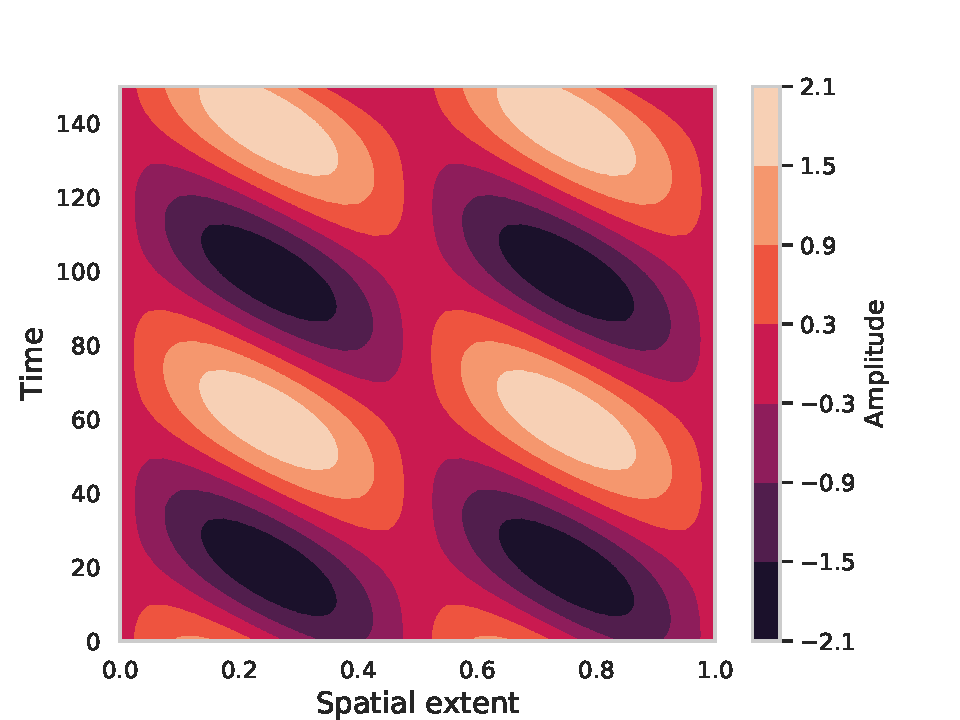
\includegraphics[width=0.5\textwidth]{hovmuller_boundedsine.pdf}
	\caption{Hov Müller diagram of a bounded Rossby wave with a initial sine wave using a explicit scheme.}
	\label{fig:hovmullerSineBounded}
\end{figure}

\begin{figure}[htbp]
	\centering
	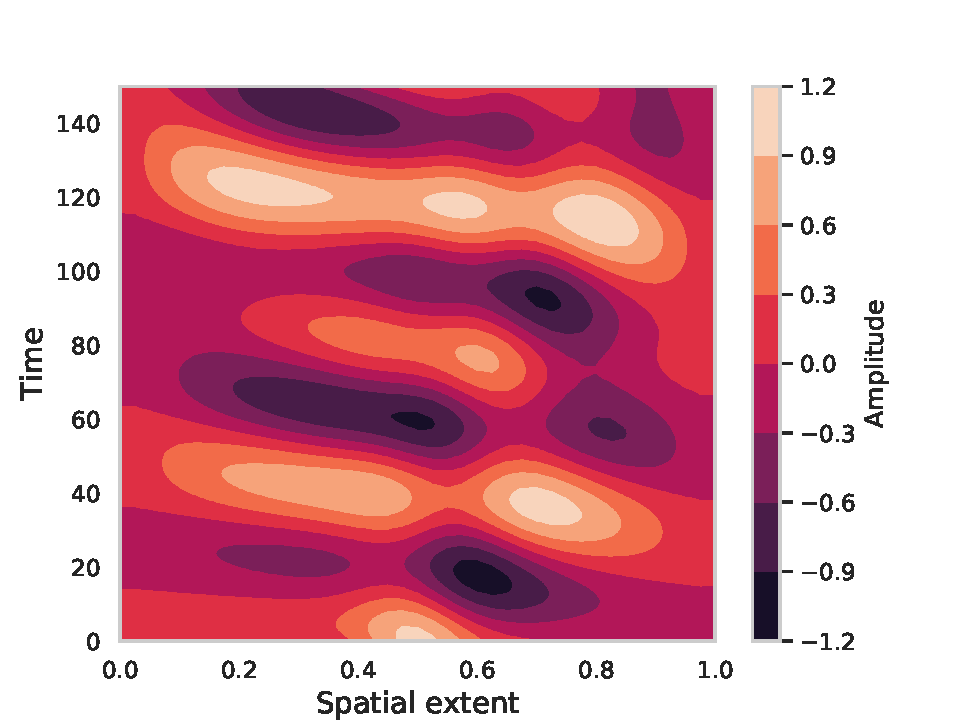
\includegraphics[width=0.5\textwidth]{hovmuller_boundedgaussian.pdf}
	\caption{Hov Müller diagram of a bounded Rossby wave initially a gaussian using a explicit scheme.}
	\label{fig:hovmullerGaussianBounded}
\end{figure}

\begin{figure}[htbp]
	\centering
	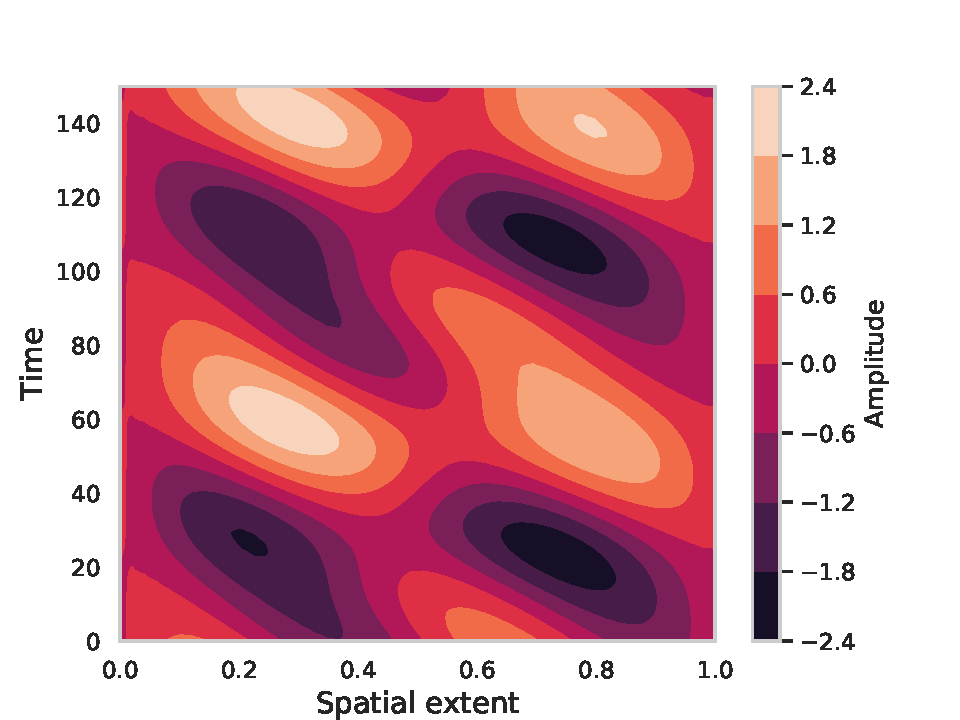
\includegraphics[width=0.5\textwidth]{hovmuller_periodicsine.pdf}
	\caption{Hov Müller diagram of a Rossby wave with periodic boundary conditions, initially a sine wave using a explicit scheme.}
	\label{fig:hovmullerSinePeriodic}
\end{figure}

\begin{figure}[htbp]
	\centering
	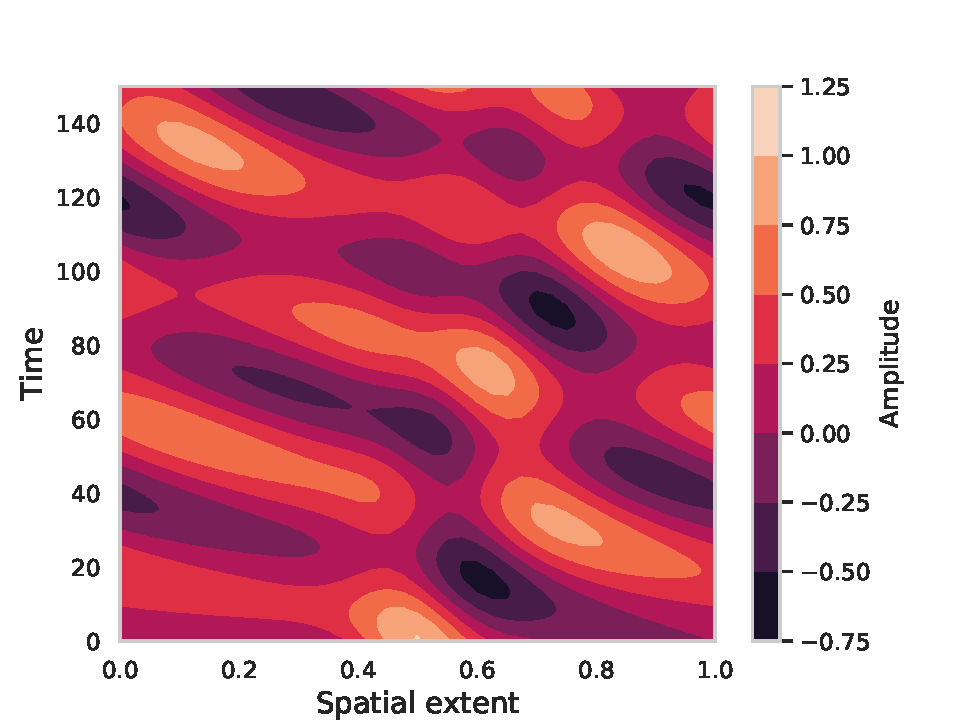
\includegraphics[width=0.5\textwidth]{hovmuller_periodicgaussian.pdf}
	\caption{Hov Müller diagram of a Rossby wave with periodic boundary conditions, initially a gaussian using a explicit scheme.}
	\label{fig:hovmullerGaussianPeriodic}
\end{figure}

\begin{table}[htbp]
	\centering
	\begin{tabular}{lrr}
		\textbf{n} & $\mathbf{{t_g}/{t_s}}$ & $\mathbf{{t_{LU}}/{t_s}}$  \\
		\midrule
		\addlinespace[0.1cm]

		10         & 2.08                                                                                          & 3.70                                                                                        \\
		$10^2$       & 1.89                                                                                          & $1.00\cdot 10^2 $                                                                                         \\
		$10^3$       & 1.48                                                                                          & $1.05 \cdot 10^4 $                                                                                        \\
		$10^4$       & 1.43                                                                                          & $1.18 \cdot 10^6$                                                                                         \\
		$10^5$       & 1.39                                                                                          & -                                                                                         \\
		$10^6$       & 1.41                                                                                          & -                                                                                        \\
		$10^7$       & 1.39                                                                                          &    -
	\end{tabular}  \caption{Ratio between CPU time for the general algorithm ($\mathbf{t_g}$), the special algorithm ($\mathbf{t_g}$) and the LU decomposition algorithm ($\mathbf{t_{LU}}$) for different matrix sizes (\textbf{n}). The LU decomposition crashed for \textbf{n} greater than $10^4$.} \label{table:time}
\end{table}

\section{Discussion}
\label{sec:discussion}

Having presented the different methods and their relative efficiency and
accuracy, we would like to discuss their uses as well as their boundaries.
We see that for our problem of solving eq. \ref{eq:gendiff}, we could construct
a very specialised and efficient algorithm because we used a 2nd order
central approximation to the 2nd derivative. This let us reduce the number of
flops by a half, and our computer should, with an optimised CPU, only have to do
half the work. In terms of accuracy, we found no significant difference between
the algorithms, and so this also means that we get the most accuracy per CPU time
with our specialised algorithm up until n=$10^{-6}$ (see Figure \ref{fig:error}).
Thus for our problem of a linear second order differential equation with
Dirichlet boundaries, this is clearly the most advantageous algorithm.

However, while the specialised algorithm is good at solving eq. \ref{eq:gendiff},
it is, as our naming suggests, not very general. There exists a wide variety of
problems that can be expressed in the form of our matrix equation, eq.
\ref{eq:matrixeq}, where the matrix A takes different forms. What we have called the general algorithm, which is almost as efficient as the specialised algorithm (see Table \ref{table:time}), can be used if the matrix A is tridiagonal.

If matrix A is not on a tridiagonal form neither our specialised nor our general algorithm can be used. In the latter case, the LU-decomposition can be useful. This comes at cost of a drastically increase in CPU run time as n increases.  
 


As we can see from Figure \ref{fig:error}, there seems to be a lower limit to the error in the specialised algorithm. From n=10 to n=$10^5$ the error decreases with a slope of about -2. From eq. \ref{eq:approx} we have that the mathematical error in our approximation goes as $h^2$, or $n^{-2}$. So our error decreases as expected from the mathematical model. 

From n=$10^5$ and up the slope increases, and from n=$10^6$ the error is increasing as n increases. This increase in the relative error is due to round-off errors caused by the computer. 

\appendix
%\onecolumn
\setcounter{equation}{0}
\renewcommand\theequation{A.\arabic{equation}}
\section*{A}
\label{sec:appendix}

Here are figures of data we gathered, but didn't end up using. Most of them are zoomed in cases, but we also include the mean magnetisation.

\begin{figure}[htbp]
	\centering
	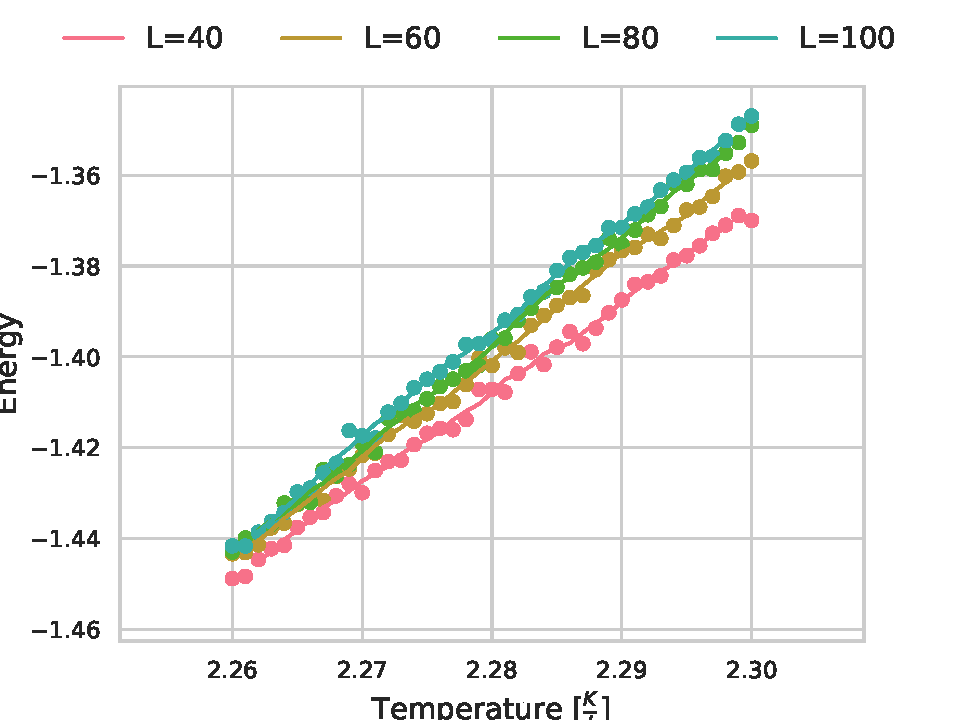
\includegraphics[width=0.5\textwidth]{Energy0001.pdf}
	\caption{Mean energy as a function of temperature $T\in[2.26, 2.3]$ for lattice sizes $L= 40, 60, 80, 100$, with a rolling mean, window size 5.}
\end{figure}

\begin{figure}[htbp]
	\centering
	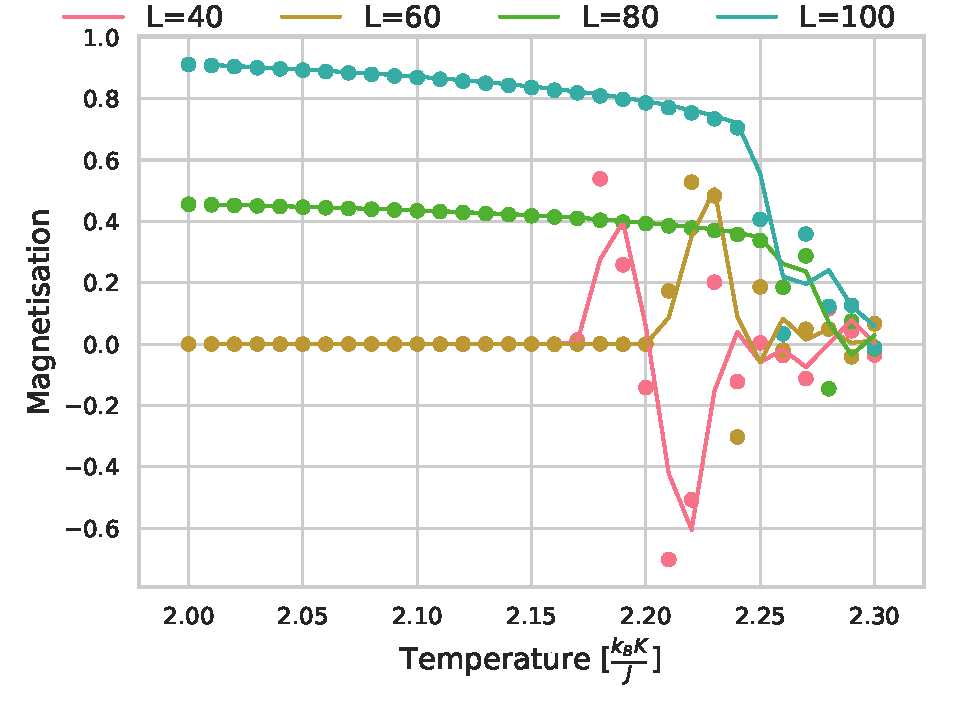
\includegraphics[width=0.5\textwidth]{Magnetisation001.pdf}
	\caption{Mean magnetisation as a function of temperature $T\in[2.0, 2.3]$ for lattice sizes $L= 40, 60, 80, 100$, with a rolling mean, window size 2.}
\end{figure}

\begin{figure}[htbp]
	\centering
	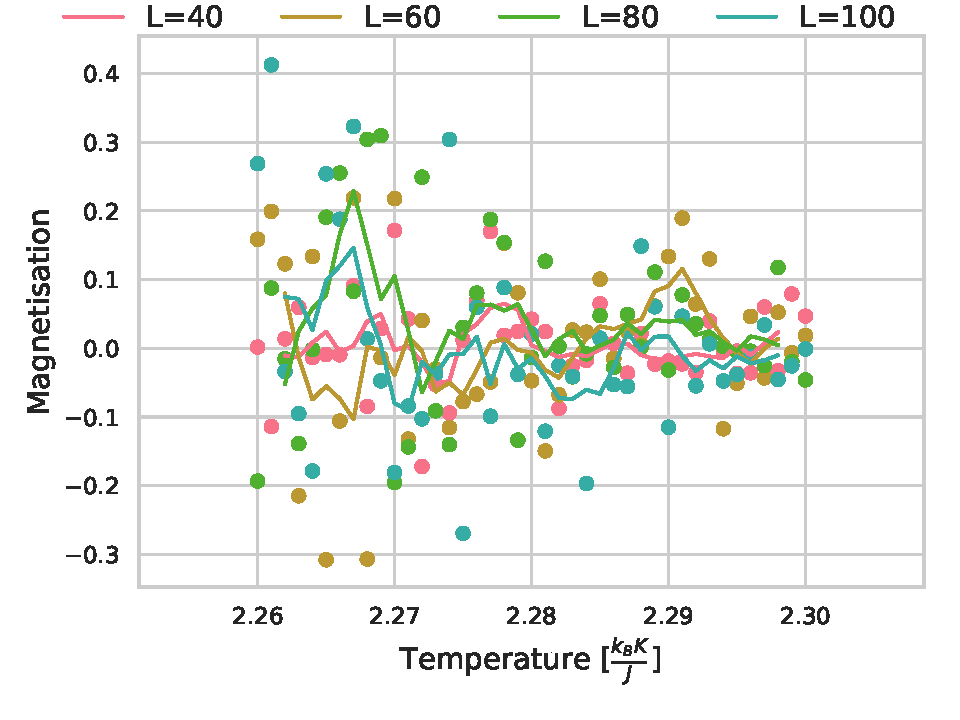
\includegraphics[width=0.5\textwidth]{Magnetisation0001.pdf}
	\caption{Mean magnetisation as a function of temperature $T\in[2.26, 2.3]$ for lattice sizes $L= 40, 60, 80, 100$, with a rolling mean, window size 5.}
\end{figure}

\begin{figure}[htbp]
	\centering
	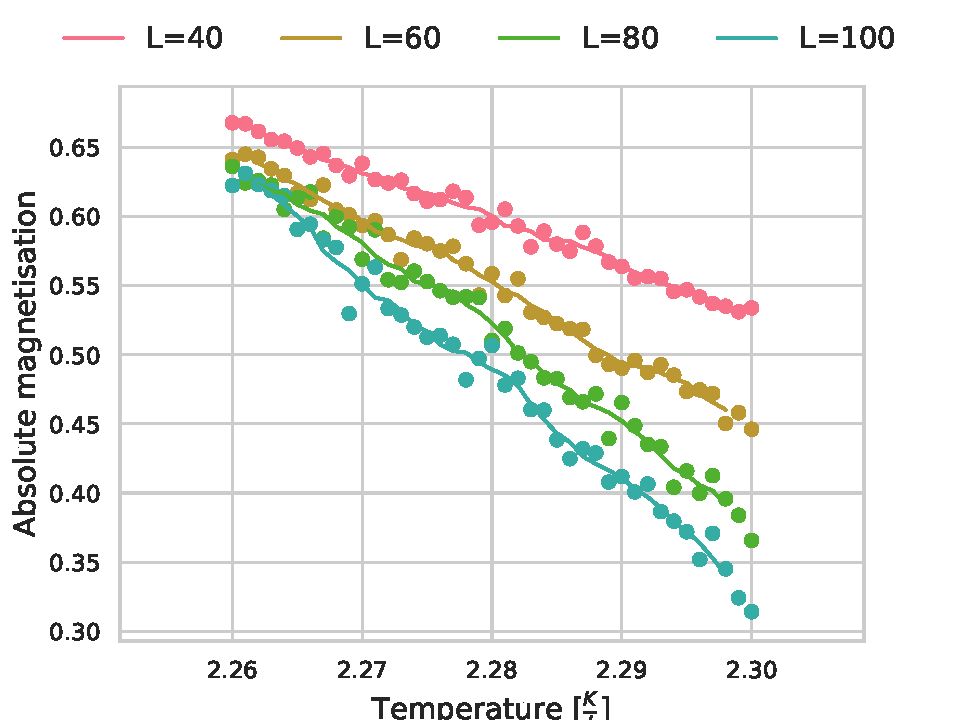
\includegraphics[width=0.5\textwidth]{Absolute_magnetisation0001.pdf}
	\caption{Absolute magnetisation as a function of temperature $T\in[2.26, 2.30]$ for lattice sizes $L= 40, 60, 80, 100$, with a rolling mean, window size 5.}
\end{figure}

\begin{figure}[htbp]
	\centering
	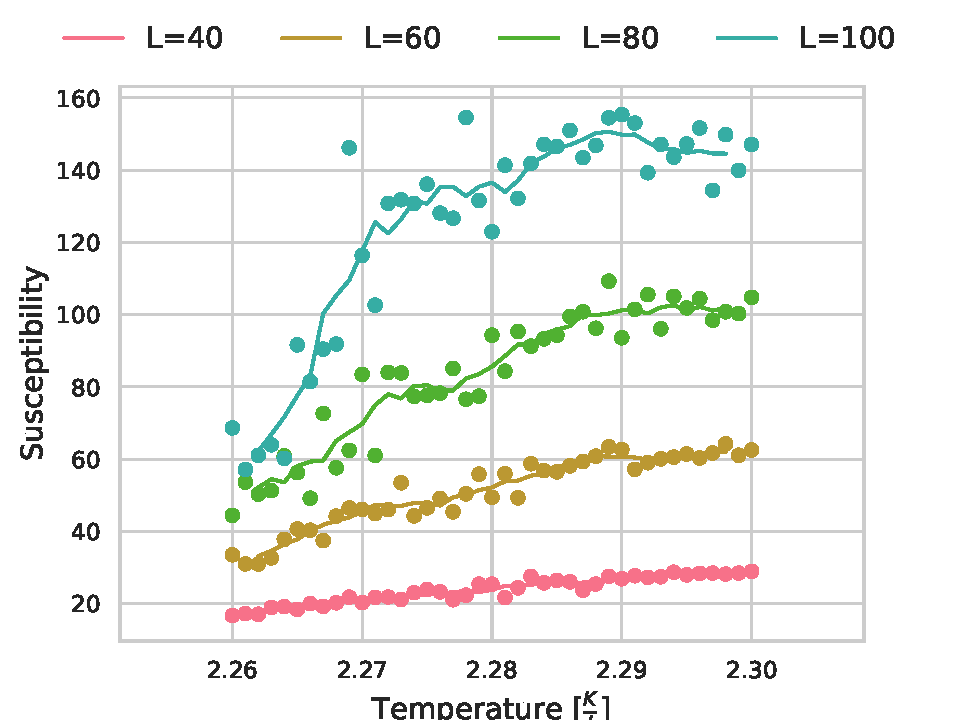
\includegraphics[width=0.5\textwidth]{Susceptibility0001.pdf}
	\caption{Susceptibility as a function of temperature $T\in[2.26, 2.30]$ for lattice sizes $L= 40, 60, 80, 100$, with a rolling mean, window size 5.}
\end{figure}


\clearpage
\printbibliography[heading=bibintoc, title=Bibliography]


\listoffigures
\listoftables

\end{document}
